\documentclass[border=6pt]{standalone}
\usepackage{amsmath}
\usepackage{amssymb}
\usepackage{tikz}
\usepackage{pgfplots}
\pgfplotsset{compat=1.18}
\usetikzlibrary{arrows.meta,calc,positioning}
\begin{document}
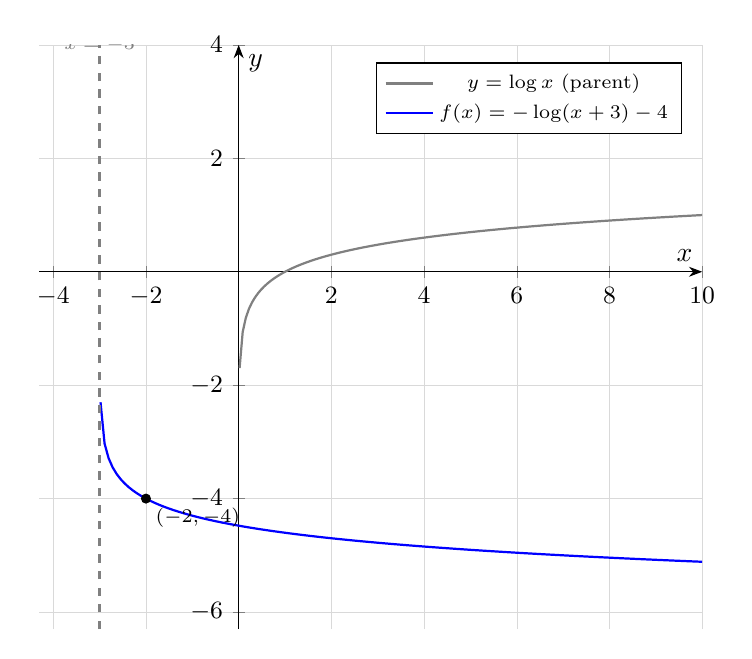
\begin{tikzpicture}
\begin{axis}[
    axis lines = middle,
    xlabel = {$x$}, ylabel = {$y$},
    grid=both,
    grid style={line width=.1pt, draw=gray!30},
    axis line style={-Stealth},
    legend style={font=\scriptsize},
    tick label style={font=\small},
    xmin=-4.3, xmax=10, ymin=-6.3, ymax=4,
    xtick={-4,-2,0,2,4,6,8,10},
    ytick={-6,-4,-2,0,2,4},
    width=10cm, height=9cm,
    legend pos=north east,
]
\addplot[domain=0.02:10, samples=150, thick, gray] {ln(x)/ln(10)};
\addlegendentry{$y=\log x$ (parent)}
\addplot[domain=-2.98:10, samples=150, thick, blue] {-(ln(x+3)/ln(10))-4};
\addlegendentry{$f(x)=-\log(x+3)-4$}
\draw[dashed, gray, thick] (axis cs:-3,-6.3) -- (axis cs:-3,4);
\node[anchor=south, font=\scriptsize, gray] at (axis cs:-3,3.7) {$x=-3$};
\addplot[only marks, mark=*, mark size=1.6pt, black] coordinates {(-2,-4)};
\node[anchor=north west, font=\scriptsize] at (axis cs:-2,-4) {$(-2,-4)$};
\end{axis}
\end{tikzpicture}
\end{document}
